\documentclass[a4paper,11pt]{report}
\usepackage[]{amsmath}
\usepackage[]{physics} % \bra, \ket etc
\usepackage{graphicx} %Pour les figures je crois
\usepackage{hyperref}
\usepackage[
    backend=biber, 
    natbib=true,
    style=numeric-comp,
    sorting=none, %Pour faire apparaitre les refs dans l'ordre
    hyperref=true
]{biblatex} %Imports biblatex package
\addbibresource{Bib_intro.bib} %Import the bibliography file

\usepackage{amssymb} %quelques symboles dont gtrsim /lesssim
\usepackage{subcaption} % package pour faire des subfigures
\usepackage{multirow} % package pour multirow/multicolumn
\usepackage{booktabs} % package pour top/mid/bottom rule
\usepackage{tcolorbox} % toujours plus de boites
\usepackage{xcolor} % Pour avoir des couleurs dans les équations


\title{}
\begin{document}
\chapter*{Introduction}

Quantum mechanics was first developed at the beginning of the 20th century to explain physical observations such as the blackbody radiation \citep{planck1900theorie} or the photoelectric effect \citep{einstein1905erzeugung}. The quantum theory was subsequently developed in the first half of the 20th century and showed great success, in particular in giving a physical framework for chemistry \citep{pauling1931nature} and leading to a microscopic understanding of matter \citep{kittel1996introduction}. In the second half of the 20th century, technological development based on the new understanding of light and matter have led to what was retroactively called the first quantum revolution \citep{thew2019focus}. Technologies developed in the 50s and 60s include the semiconductor transistor \citep{bardeen1948transistor}, the laser \citep{maiman1960stimulated}, and nuclear magnetic resonance \citep{abragam1961principles} which have since revolutionized the fields of information science, global communications and medical imaging. 

A new field of quantum technology has emerged in the last two decades. This ``second quantum revolution" differs from the first one in the usage of individual quantum systems, such as single photons \citep{gleyzes2007quantum}, atoms \citep{neuhauser1980localized} or electrons \citep{peil1999observing}, which have properties that can not be emulated by larger classical systems. These properties include quantum entanglement, superposition or measurement and form the basis of the newly formed quantum information science \citep{nielsen2002quantum, vedral2006introduction, hayashi2006quantum}. 

Central to quantum information science is the idea of quantum bits or qubits \citep{schumacher1996sending}, which are the building blocks of quantum information in analogy to the bits of classical information theory. Physical implementation of a qubit could be any quantum system with two well defined quantum states, as long as these states can be initialized, manipulated and readout \citep{divincenzo2000physical}. Popular qubit candidates include superconducting circuits \citep{nakamura1999coherent, orlando1999superconducting}, photons \citep{bennett1992quantum, zhong2020quantum}, quantum dots \citep{veldhorst2014addressable, zajac2018resonantly}, trapped ions \citep{friis2018observation, wright2019benchmarking} and single crystal defects \citep{jelezko2006single, baranov2011silicon, zhong2015optically}.

Defects in large band gap crystals are sometimes referred to as artificial atoms \citep{buluta2011natural}, as the localized wave function of the electrons surrounding the impurity  give rise to discrete energy levels similar to that of an atom. Of all the possible crystals and defects, the most studied defect for quantum applications is the negatively charged nitrogen-vacancy center in diamond \citep{aharonovich2016solid, de2021materials}, often abbreviated to ``NV center". Although this defect had been known and correctly identified almost 50 years ago \citep{davies1976optical}, interest in the NV center really sparked after it was first isolated in 1997 \citep{gruber1997scanning}. The detection of single NV centers proved that NV centers fluoresce brightly \citep{gruber1997scanning}, are photostable \citep{kurtsiefer2000stable}, and that their electronic spin can be polarized and readout optically \citep{jelezko2004observation}, making them an promising solid state qubit.

Since then, single NV centers have been successfully used to create quantum entanglement over several km \citep{hensen2015loophole}, to store quantum information at room temperature for more than one second \citep{maurer2012room}, to detect single proteins via nuclear magnetic resonance \citep{lovchinsky2016nuclear}, and for many other applications in quantum communication \citep{wehner2018quantum}, quantum computing \citep{de2021materials} or quantum sensing \citep{degen2017quantum}.

As the interest in single NV center grew, diamond synthesis improved significantly \citep{achard2020chemical, barry2020sensitivity, edmonds2020generation}  which benefited not only single NV centers but also NV center ensemble. While single NV center are required for most quantum information processes \citep{ladd2010quantum}, several other applications benefit from a greater concentration of defects and are therefore more suited to operate with NV centers ensemble. Four of these applications are pictured in Fig. \ref{shema introduction}.

\begin{figure}[h!]
\centering
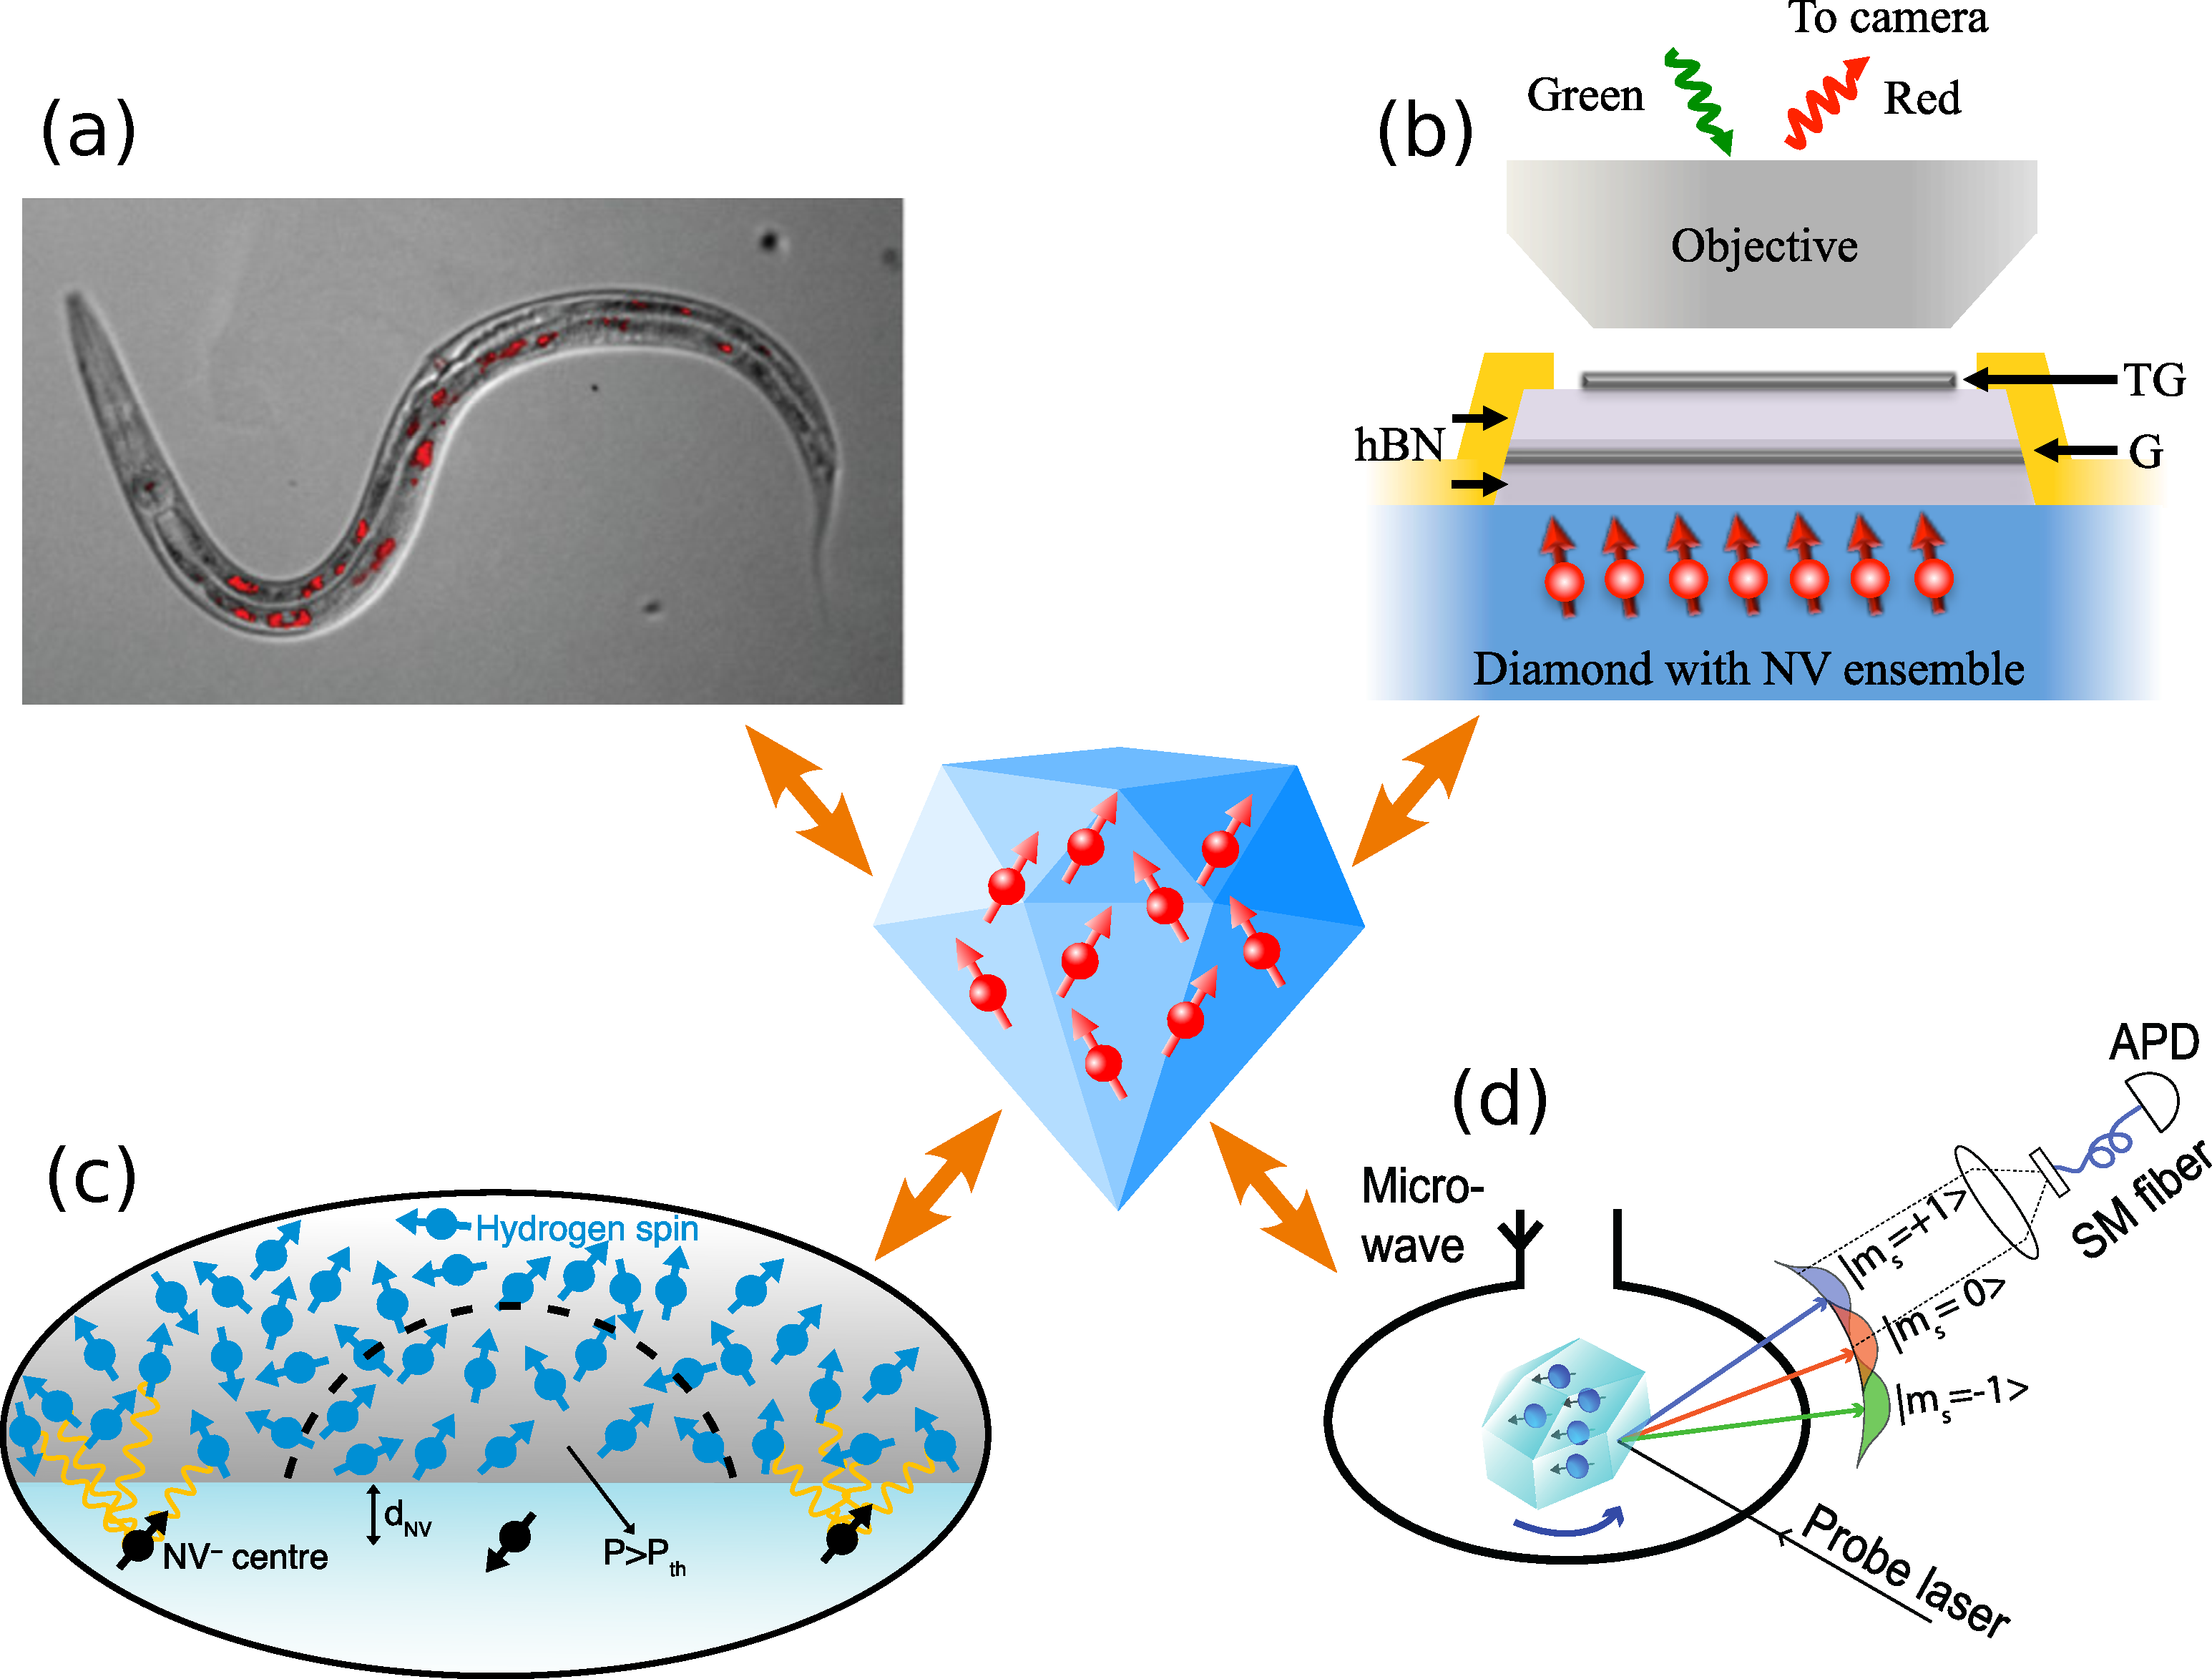
\includegraphics[width=.9\textwidth]{Figures/Fig_intro}
\caption{Example of applications with dense ensemble of NV centers. (a) In vivo nanodiomond biomarkers (from \citep{mohan2010vivo}). (b) Quantum sensing with NV ensemble (from \citep{ku2020imaging}). (c) Dynamic nuclear polarization of an external spin bath (from \citep{healey2021polarization}). (d) Spin mechanics with trapped micro diamonds (from \citep{delord2020spin}).}
\label{shema introduction}
\end{figure}

The first application for NV center ensemble is the use of nano or micro diamonds as fluorescent biomarkers \citep{fu2007characterization, mohan2010vivo}. NV centers are good candidates for biomarkers as they emit a bright and stable photoluminesecence, and because diamond nanocrystals present low toxicity \citep{schirhagl2014nitrogen}. Some applications also use the spin degree of freedom of the NV centers, either to perform background free fluorescence microscopy \citep{chapman2013background} or to monitor the angular motion of the nanodiamonds \citep{mcguinness2011quantum, feng2021association}. For most of these applications, NV ensemble provide a better visibility than single NV centers and are therefore preferred.

The second NV ensemble application is for quantum sensing \citep{degen2017quantum}. NV centers are predominantly used as magnetic field sensors \citep{rondin2014magnetometry, barry2020sensitivity}, although they can also detect electric fields \citep{dolde2011electric, michl2019robust}, temperature \citep{acosta2010temperature, kucsko2013nanometre} ,crystal strain \citep{ovartchaiyapong2014dynamic, doherty2014electronic} or rotation \citep{ledbetter2012gyroscopes, ajoy2012stable}. Both single and ensemble of NV centers can be used for sensing: single centers offer unmatched spatial resolution \citep{mitchell2020colloquium} down to a few nm \citep{lovchinsky2016nuclear}, while ensemble provide better sensitivities \citep{wolf2015subpicotesla, barry2020sensitivity}. 

The third NV ensemble application is nuclear magnetic resonance (NMR) dynamical nuclear polarization \citep{eills2022spin}. Dynamic nuclear polarization consists in increasing the nuclear polarization of a sample by transferring electron polarization to the nuclei bath \citep{abragam1978principles}. Because the NV electronic spin can be optically polarized at room temperature, micro and nano diamonds containing NV centers are promising candidates as hyperpolarization agents \citep{tetienne2021prospects}. Nuclear polarization of spins inside the diamond lattice was demonstrated with single NV centers \citep{jacques2009dynamic, smeltzer2009robust} and NV ensemble \citep{king2015room, scheuer2016optically, schwartz2018robust}. Polarization transfer to nuclear spins outside of the diamond is an ongoing challenge \citep{eills2022spin, healey2021polarization}, but dense NV ensemble are believed to be necessary to achieve high external polarization \citep{tetienne2021prospects, rizzato2022polarization}.

Finally, the fourth NV ensemble application is the recent field of spin mechanics \citep{perdriat2021spin}. Similarly to optomechanics \citep{aspelmeyer2014cavity}, the goal of spin mechanics is to couple a quantum system to the mechanical degree of freedom of a macroscopic object. Strong coupling between single NV center and an external mechanical oscillators has been observed \citep{rabl2009strong, kolkowitz2012coherent}, but coupling between NV centers and the motion of the diamond has so far only been achieved with dense NV ensemble \citep{delord2020spin, pellet2021magnetic, perdriat2022angle}. Coupling several NV centers to the same mechanical oscillator could also lead to interesting magnetic phase transitions \citep{wei2015magnetic, ma2017proposal}.
   
Most of the NV ensemble experiments discussed previously work under the assumption that the ensemble is constituted of $N$ independent single NV centers. However, as often in physics, \textit{more is different} \citep{anderson1972more}. Interaction between the NV center themselves or with their environment can lead to significantly different behavior between ensemble and single spins. These difference include a modification of the charge state dynamics \citep{giri2018coupled} and of the spin dynamics \citep{dobrovitski2008decoherence, jarmola2012temperature, mrozek2015longitudinal, choi2017depolarization}, as well as the apparition of exotic phenomena such as time crystal phase \citep{choi2017observation}, Anderson localization \citep{kucsko2018critical} or superradiance \citep{bradac2017room, angerer2018superradiant}. 

The work presented in this manuscript focuses on dipolarly coupled dense ensemble of NV centers. More specifically, we look at spin polarization exchange between the NV centers themselves and with their environment. Polarization exchange (flip-flop, spin diffusion, cross-relaxation, ...) in dense ensemble of spins has been abundantly studied in the context of NMR \citep{abragam1978principles} and spintronics \citep{vzutic2004spintronics}. Because NV centers tend to be relatively dilute, the question of spin exchange between between NV themselves \citep{choi2017depolarization} or with their environment \citep{hall2016detection} has only recently been addressed. However, as samples with higher NV concentration become available \citep{acosta2009diamonds, tallaire2020high, shenderova2019synthesis}, these aspects are becoming more and more relevant.

The goal of this present work is both to better understand the physics of dense NV ensemble, which is crucial for many of the NV ensemble applications cited previously, and to exploit some of these many-body properties for new applications.

\bigskip
This manuscript is organized in the following way:

\medskip
The first chapter introduces the theoretical and experimental concepts used in this manuscript. This includes a brief overview of diamond and NV centers fabrication processes, the physics of single NV centers and a presentation of magnetic dipole-dipole interaction and cross-relaxation.

The second chapter covers the observation of cross-relaxation between NV centers and other spin impurities in CVD-grown diamond. We use measurements on the NV centers to identify these impurities and to quantify some of their attributes. Most of the results of this chapter have been published in  \citep{pellet2021optical} and \citep{ngambou2022improving}.

The third chapter focuses on the dipole-dipole mediated spin relaxation within dense ensemble of NV centers. Following the work presented in \citep{choi2017depolarization}, we introduce the concept of NV-flutcuator to explain this phenomenon and present experimental and theoretical results solidifying this hypothesis. The results of this chapter have been partly published in \citep{pellet2022spin} and \citep{pellet2021magnetic}.

Finally, the fourth chapter presents a study on NV-NV dipolar relaxation under low magnetic field. This chapter covers both the rich physics of NV centers under low magnetic field, and a potential application of the low field depolarization as a new magnetometry protocol, as well as comparisons with other NV magnetometry protocols. The results of this chapter have in large part been published in \citep{pellet2022spin}.

\printbibliography
\end{document}